%% Thin is an attempt at a generic preamble that can be called instead of copies 
%% a bunch of times. Any specific/minor document tweaks can be added to the main document
%% preamble and should therefore override and/or add to these settings.
%%---------------------------------------------------------------------------%%

%%------   page format
% set text encoding to utf-8
\usepackage[utf8]{inputenc}

% page margins
\usepackage[top=0in, bottom=0in, left=0in, right=0in]{geometry}
% \usepackage[top=0.5in, bottom=0.5in, left=1in, right=1in]{geometry}

% contrl end of line wrap/hyphenation 
\usepackage{ragged2e}

% More granular control over title format of part, section, subsection, paragragh ...
\usepackage{titlesec}
% Custom section spacing and formatting examples:
% \titleformat{\part}{\Huge\scshape\filcenter}{}{1em}{}
% \titleformat{\section}{\Large\bf\raggedright}{}{1em}{}[{\titlerule[2pt]}]
% \titlespacing{\section}{0pt}{3pt}{7pt}
% \titleformat{\subsection}{\large\bfseries\centering}{}{0em}{\underline}[\rule{3cm}{.2pt}]
% \titlespacing{\subsection}{0pt}{7pt}{7pt}

% list formatting
% to use the three basic list in line: just add the package option inline and then the 
% environments enumerate*, itemize* and description*.
\usepackage{enumitem} 

%%------ LaTeX mechanics

 % allows compile of only subfile
\usepackage{subfiles}

% branch logic
\usepackage{xifthen}

%%------   debug/development
\usepackage{blindtext} % Dummy text and tools 
%\Blindtext [2] [1] % two paragraphs 1 textblock

 % adds multiline comments
\usepackage{comment}
% \begin{comment} ... \end{comment}

%%------   math tools
\usepackage{mathtools} % new, contains amsmath
\usepackage{upgreek} % better looking Greek

%%------   image/figure tools
\usepackage{graphicx}
\graphicspath{ {../images/} } %   implies images dir in current dir
\usepackage{wrapfig}
\usepackage[font=scriptsize,labelfont=bf]{caption}

\usepackage{background}

% this took some playing around with to get the positioning right
% I think the origin is the top left corner of the page now
\backgroundsetup{
   scale=1,
   position={0in, 0in},
   anchor=topleft,
   nodeanchor= north west,
   hshift=-1in,
   vshift=1in,
   angle=0,
   opacity=0.5,
  % contents={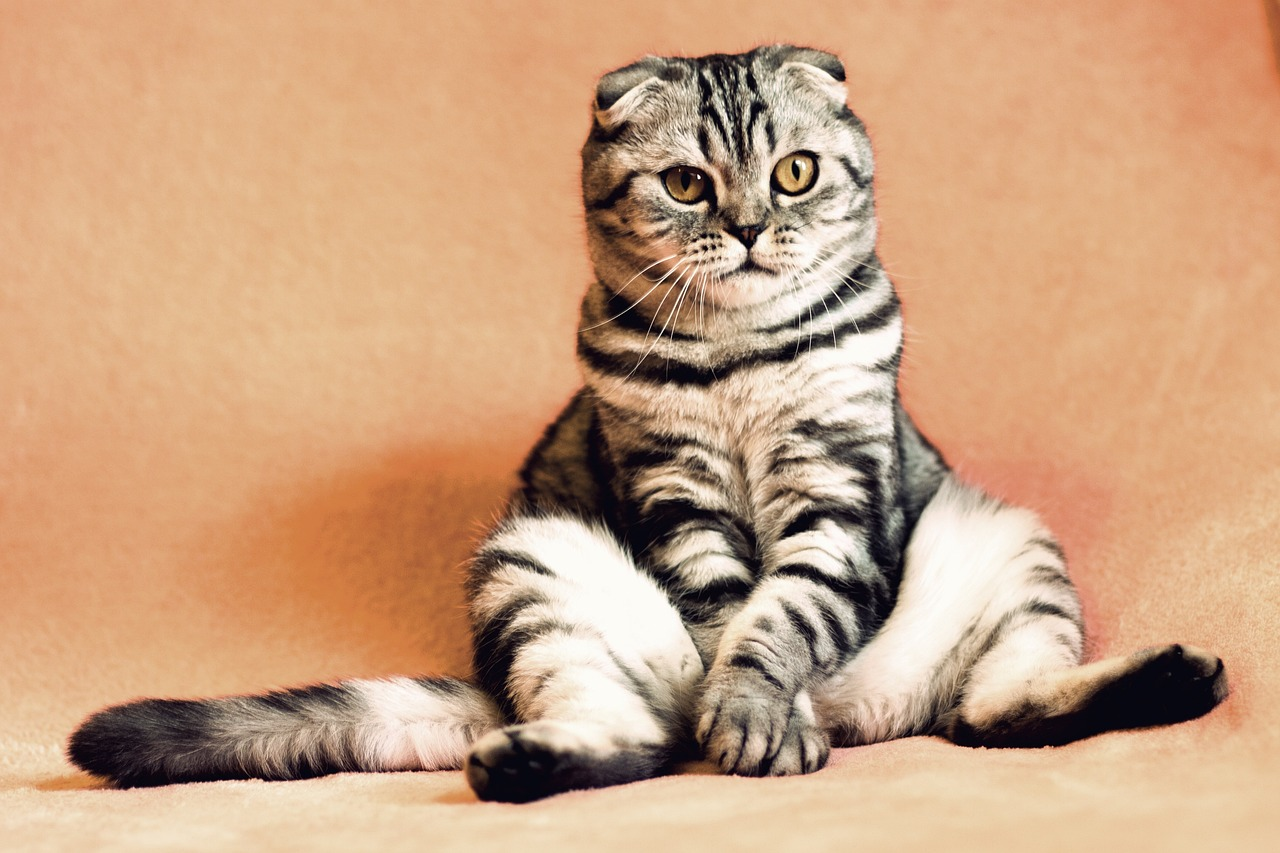
\includegraphics[width=\paperwidth,height=\paperheight]{cat.jpg}}
  % contents={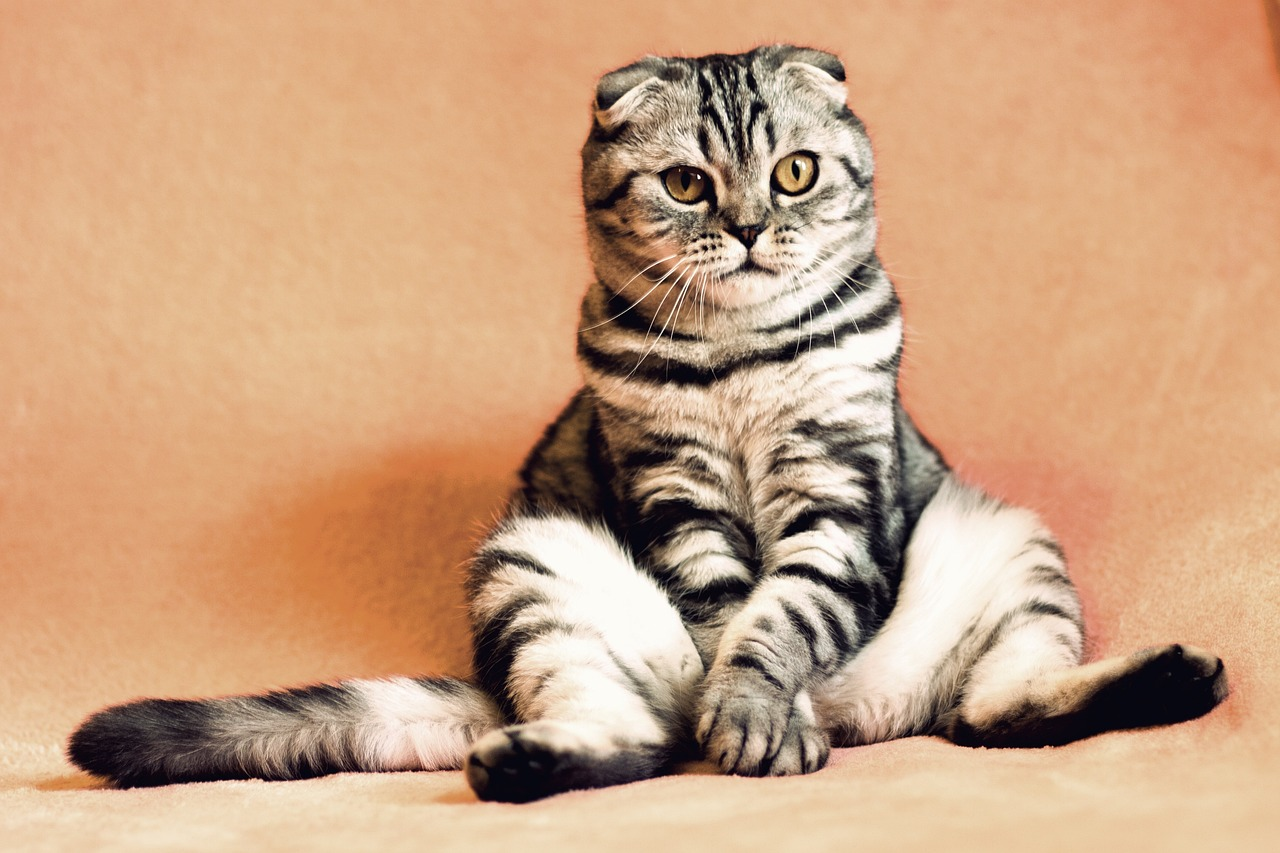
\includegraphics[width=8.5in, height=11in]{cat.jpg}}
  contents={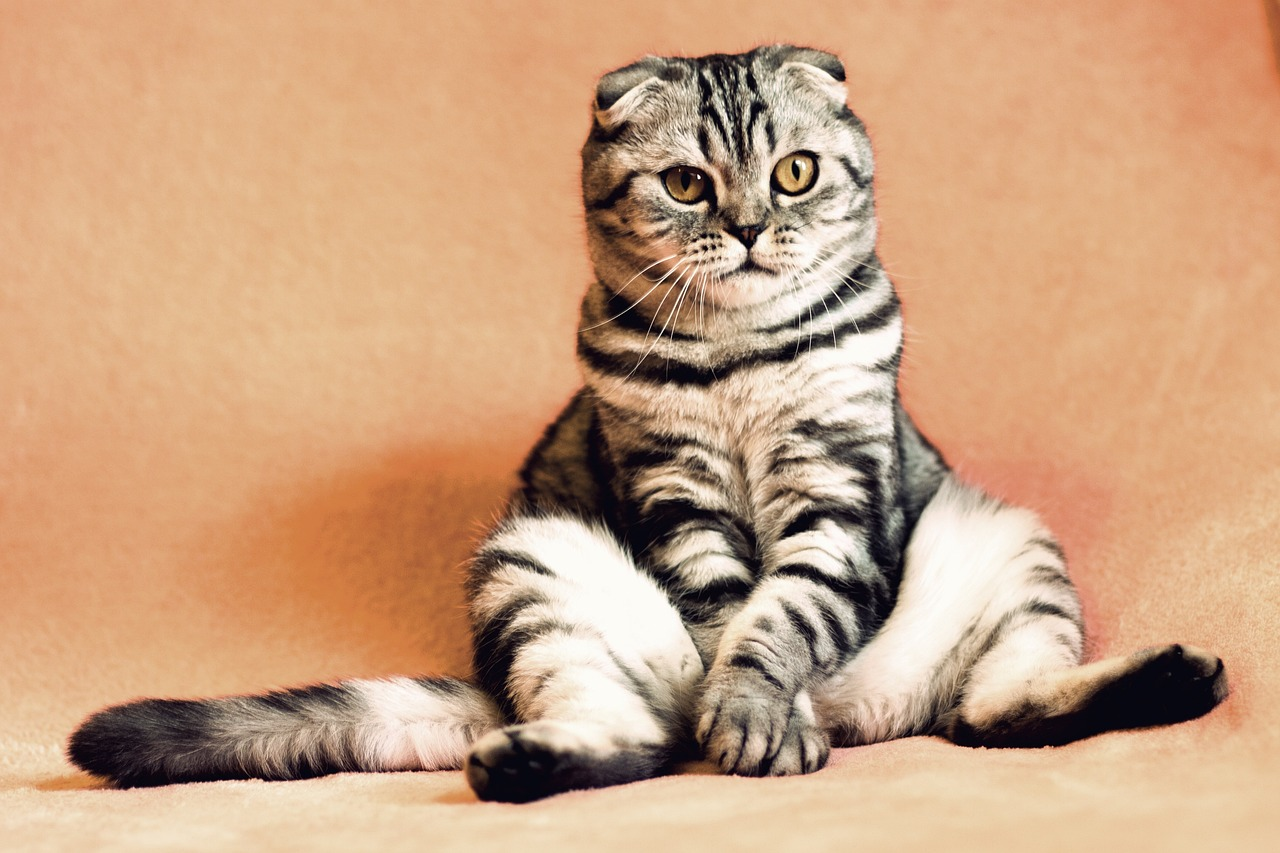
\includegraphics[width=8.5in]{cat.jpg}}
}
% \backgroundsetup{
% % option                  % Possible Values           % Default Value
%   pages=all,              % <all|some>                % all
%   firstpage=false,        % <true|false>              % false
%   placement=center,       % <center|top|bottom>       % center
%   contents={Draft},       % text, image, Tikz, etc.   % Draft                % Draft
%   color=red!45,           % Any valid color           % red!45
%   angle=60,               % Any -360 to 360           % 60, for center
%                                                       % 0, for top and bottom
%   opacity=0.5             % Any 0 to 1                % 0.5
%   scale=1,                % Any positive value        % 15 for center
%                                                       % 8 for top and bottom
%   position={page.center}, % Any valid node            % current page.center for center
%                           % for placement             % current page.north for top
%                                                       % current page.south for bottom
%   anchor={},              % Any implified value       % empty for center
%                           % node for anchor           % below for top
%                                                       % above for bottom
%   nodeanchor=center,      % Any value for node        % center
%                           % anchor                    % below for top
%                                                       % above for bottom
%   hshift=0pt              % Any length.               % 0pt
%   vshift=0pt              % Any length.               % 0pt
% }

%%------ figure/diagram tools

%%------ table tools

%%------
